\section{The Linear Intuition}

% ====================================================
% --- Slide 1: Thiết lập trực giác (Không có toán) ---
% ====================================================
\begin{frame}{Bài toán phân loại trên mặt phẳng}
  \begin{columns}
    \begin{column}{0.4\textwidth}
      \begin{itemize}
        \item Cho hai nhóm dữ liệu: \textcolor{blue}{Nhóm A} và \textcolor{red}{Nhóm O}.
        \item Mục tiêu: Tìm một \textbf{đường ranh giới} để phân tách chúng.
        \item Có \textbf{vô số} cách vẽ đường thẳng.
        \item \textit{Vậy đâu là ranh giới hợp lý nhất?}
      \end{itemize}
    \end{column}
    
    \begin{column}{0.6\textwidth}
      \centering
      \begin{tikzpicture}[scale=1.2]
        % Vẽ khung trục tọa độ nhẹ nhàng
        \draw[->, gray!50] (-0.5,0) -- (5,0) node[right] {$x_1$};
        \draw[->, gray!50] (0,-0.5) -- (0,4) node[above] {$x_2$};

        % Nhóm A (màu xanh)
        \filldraw[blue] (3,3) circle (2pt);
        \filldraw[blue] (4,2.5) circle (2pt);
        \filldraw[blue] (2.5,4) circle (2pt);
        \filldraw[blue] (4,3.5) circle (2pt);
        \filldraw[blue] (3.2,2.8) circle (2pt);

        % Nhóm O (màu đỏ)
        \filldraw[red] (1,0.5) rectangle (1.2,0.7);
        \filldraw[red] (2,-0.2) rectangle (2.2,0);
        \filldraw[red] (0.5,1) rectangle (0.7,1.2);
        \filldraw[red] (1.8,0.8) rectangle (2.0,1.0);
        \filldraw[red] (0.8,1.8) rectangle (1.0,2.0);
      \end{tikzpicture}
    \end{column}
  \end{columns}
\end{frame}

% ====================================================
% --- Slide 2: Khớp nối trực giác vào Công thức ---
% ====================================================
\begin{frame}{Ý tưởng cốt lõi: Đường ranh giới an toàn nhất}
  \begin{columns}
    \begin{column}{0.4\textwidth}
      \textbf{Làm sao để chọn đường tốt nhất?}
      \vspace{0.3cm}
      \begin{enumerate}
        \item Hãy tưởng tượng một \textbf{"con đường"} càng rộng càng tốt để phân tách hai nhóm.
        \item \textbf{Đường ranh giới} sẽ nằm chính giữa con đường đó.
        \item Những điểm nằm sát mép đường được gọi là \textbf{Support Vectors} (Điểm trụ cột).
      \end{enumerate}
      \vspace{0.3cm}
      \textbf{Kết luận:} Đường thẳng \textit{an toàn nhất} là đường có \textbf{lề đường rộng nhất}.
    \end{column}
    
    \begin{column}{0.6\textwidth}
      \centering
      \begin{tikzpicture}[scale=1.2, >=stealth]
        % Trục tọa độ
        \draw[->, gray!50] (-0.5,0) -- (5,0);
        \draw[->, gray!50] (0,-0.5) -- (0,4);

        % Dữ liệu lớp Xanh
        \filldraw[blue] (3,3) circle (2pt);
        \filldraw[blue] (4,2.5) circle (2pt);
        \filldraw[blue] (2.5,4) circle (2pt);
        \filldraw[blue] (4,3.5) circle (2pt);
        \filldraw[blue] (3.2,2.8) circle (2pt);
        
        % Support Vector Xanh (nằm sát mép)
        \filldraw[blue] (2,3.5) circle (2.5pt);
        \draw[blue, thick] (2,3.5) circle (5pt);
        \node[blue] at (1.5, 3.8) {SV};

        % Dữ liệu lớp Đỏ
        \filldraw[red] (1,0.5) rectangle (1.2,0.7);
        \filldraw[red] (2,-0.2) rectangle (2.2,0);
        \filldraw[red] (0.5,1) rectangle (0.7,1.2);
        \filldraw[red] (1.8,0.8) rectangle (2.0,1.0);
        
        % Support Vector Đỏ (nằm sát mép)
        \filldraw[red] (1.4,1.4) rectangle (1.6,1.6);
        \draw[red, thick] (1.5,1.5) circle (5pt);
        \node[red] at (1.0, 1.0) {SV};

        % Đường ranh giới chính giữa
        \draw[ultra thick, DarkBlue] (0.2, 3.3) -- (3.8, -0.3) node[below right] {\footnotesize Ranh giới};

        % Đường biên (Margin)
        \draw[dashed, thick, DarkBlue!60] (0, 2.5) -- (3, -0.5);
        \draw[dashed, thick, DarkBlue!60] (1, 4.5) -- (4.5, 1.0);

        % Mũi tên chỉ khoảng cách Margin
        \draw[<->, black, thick] (1.3, 2.2) -- (2.3, 3.2) node[midway, sloped, above] {\small Margin};
      \end{tikzpicture}
    \end{column}
  \end{columns}
\end{frame}

% ================================================
% SLIDE 3
% ================================================
\begin{frame}{Biểu diễn ranh giới trong không gian 2 chiều}
  \begin{columns}
    \begin{column}{0.45\textwidth}
      Một đường thẳng trên mặt phẳng $\mathbb{R}^2$ có dạng:
      \[
      w_1 x_1 + w_2 x_2 + b = 0
      \]
      \vspace{0.2cm}
      \textbf{Ý nghĩa các thành phần:}
      \begin{itemize}
        \item $\vec{w} = (w_1, w_2)$: vector \textbf{vuông góc} với đường thẳng, quyết định \textit{hướng}.
        \item $b$: điều chỉnh \textit{vị trí} (tịnh tiến song song).
      \end{itemize}
      \vspace{0.3cm}
      Khi thay tọa độ điểm $A(x_1^A, x_2^A)$ vào vế trái, dấu của kết quả cho biết điểm nằm \textit{phía nào} của đường thẳng.
    \end{column}
    \begin{column}{0.55\textwidth}
      \centering
      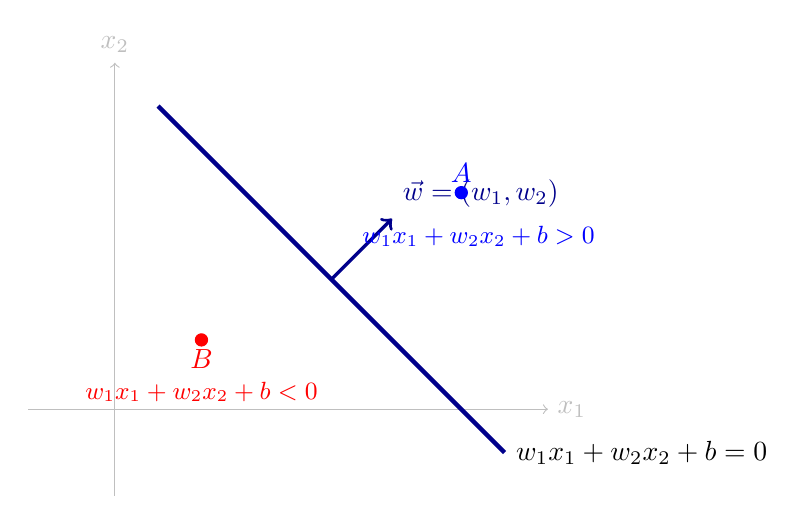
\begin{tikzpicture}[scale=1.1]
        \draw[->, gray!50] (-1,0) -- (5,0) node[right] {$x_1$};
        \draw[->, gray!50] (0,-1) -- (0,4) node[above] {$x_2$};
        % Đường thẳng
        \draw[ultra thick, DarkBlue] (0.5,3.5) -- (4.5,-0.5) node[right, text=black] {$w_1 x_1 + w_2 x_2 + b = 0$};
        % Vector pháp tuyến
        \draw[->, very thick, DarkBlue] (2.5,1.5) -- (3.2,2.2) node[above right] {$\vec{w} = (w_1, w_2)$};
        % Điểm minh họa
        \filldraw[blue] (4,2.5) circle (2pt) node[above] {$A$};
        \filldraw[red] (1,0.8) circle (2pt) node[below] {$B$};
        % Ghi chú dấu
        \node[blue] at (4.2,2) {\small $w_1 x_1 + w_2 x_2 + b > 0$};
        \node[red] at (1,0.2) {\small $w_1 x_1 + w_2 x_2 + b < 0$};
      \end{tikzpicture}
    \end{column}
  \end{columns}
\end{frame}

% ========================================================
% Slide 4: Toán học tổng quát
% ========================================================
\begin{frame}{Tổng quát hóa: Siêu phẳng và bài toán}
  \begin{block}{Từ 2D đến không gian $d$ chiều}
    Trong không gian nhiều chiều, ranh giới là một \textbf{siêu phẳng}:
    \[
    \bm{w}^T \bm{x} + b = 0
    \]
    với $\bm{w} \in \mathbb{R}^d$, $b \in \mathbb{R}$.
  \end{block}

  \begin{columns}
    \begin{column}{0.5\textwidth}
      \textbf{Khoảng cách từ điểm đến siêu phẳng:}
      \[
      d = \frac{|\bm{w}^T \bm{x} + b|}{\|\bm{w}\|}
      \]
      \vspace{0.2cm}
      \textbf{Mục tiêu phân loại:}
      \begin{itemize}
        \item Điểm lớp xanh (+1): $\bm{w}^T \bm{x} + b \geq +1$
        \item Điểm lớp đỏ (-1): $\bm{w}^T \bm{x} + b \leq -1$
      \end{itemize}
      $\Rightarrow y_i (\bm{w}^T \bm{x}_i + b) \geq 1, \forall i$
    \end{column}
    \begin{column}{0.5\textwidth}
      \centering
      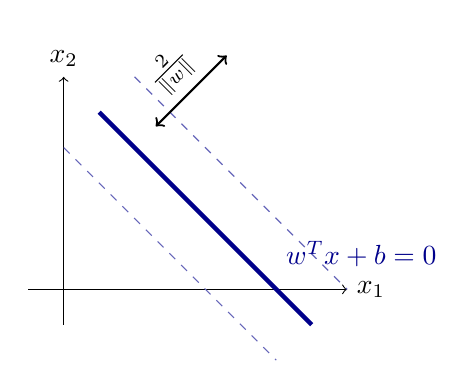
\begin{tikzpicture}[scale=0.9]
        \draw[->] (-0.5,0) -- (4,0) node[right] {$x_1$};
        \draw[->] (0,-0.5) -- (0,3) node[above] {$x_2$};
        \draw[ultra thick, DarkBlue] (0.5,2.5) -- (3.5,-0.5);
        \draw[dashed, DarkBlue!60] (0,2) -- (3,-1);
        \draw[dashed, DarkBlue!60] (1,3) -- (4,0);
        \draw[<->, thick] (1.3,2.3) -- (2.3,3.3) node[midway, above, sloped] {$\frac{2}{\|\bm{w}\|}$};
        \node[DarkBlue] at (4.2,0.5) {$\bm{w}^T\bm{x}+b=0$};
      \end{tikzpicture}
    \end{column}
  \end{columns}
\end{frame}

% ================================================
% Phát biểu mô hình
% ================================================
\begin{frame}{Tổng quát mô hình}
  \textbf{Giả định của mô hình:}
  \begin{itemize}
    \item Dữ liệu huấn luyện $\{(\bm{x}_i, y_i)\}_{i=1}^n$ với $\bm{x}_i \in \mathbb{R}^d$, nhãn $y_i \in \{-1, +1\}$.
    \item \textbf{Tuyến tính khả tách}: Tồn tại ít nhất một siêu phẳng phân tách hoàn toàn hai lớp.
  \end{itemize}

  \vspace{0.3cm}
  \textbf{Mô hình SVM (dạng hard-margin):}
  \begin{block}{Siêu phẳng phân loại}
    \[
    f(\bm{x}) = \bm{w}^T \bm{x} + b
    \]
    \begin{itemize}
      \item Nếu $f(\bm{x}) \ge 0$: dự đoán lớp $+1$ (xanh)
      \item Nếu $f(\bm{x}) < 0$: dự đoán lớp $-1$ (đỏ)
    \end{itemize}
  \end{block}
\end{frame}

\begin{frame}{Tổng quát mô hình}
  \begin{alertblock}{Điều kiện phân loại đúng với margin}
    Để đảm bảo mọi điểm nằm \textbf{ngoài hoặc trên mép lề}, ta yêu cầu:
    \[
    y_i \cdot (\bm{w}^T \bm{x}_i + b) \geq 1, \quad \forall i = 1,\dots,n
    \]
  \end{alertblock}
\end{frame}

% ==============================================
% Điều kiện sử dụng
% ==============================================
\begin{frame}{Điều kiện sử dụng của SVM với biên cứng}
  \begin{columns}
    \begin{column}{0.4\textwidth}
      \textbf{Giả định lý tưởng:}
      \begin{itemize}
        \item Hai lớp \textbf{hoàn toàn tách biệt}.
        \item Không có điểm nhiễu (outlier).
        \item Không có điểm bị gán nhãn sai.
      \end{itemize}
      \vspace{0.3cm}
      Khi đó, tồn tại siêu phẳng phân tách với margin cực đại một cách \textbf{hoàn hảo}.
    \end{column}
    \begin{column}{0.6\textwidth}
      \centering
      \begin{tikzpicture}[scale=1.1]
        \draw[->, gray!50] (-1,0) -- (5,0) node[right] {$x_1$};
        \draw[->, gray!50] (0,-1) -- (0,4) node[above] {$x_2$};
        % Dữ liệu sạch
        \filldraw[blue] (3,3) circle (2pt); \filldraw[blue] (4,2.5) circle (2pt);
        \filldraw[blue] (2.5,4) circle (2pt); \filldraw[blue] (4,3.5) circle (2pt);
        \filldraw[red] (1,0.5) rectangle (1.2,0.7); \filldraw[red] (2,-0.2) rectangle (2.2,0);
        \filldraw[red] (0.5,1) rectangle (0.7,1.2); \filldraw[red] (1.8,0.8) rectangle (2.0,1.0);
        % Siêu phẳng
        \draw[ultra thick, DarkBlue] (0.2,3.3) -- (3.8,-0.3);
        \draw[dashed, DarkBlue!60] (0,2.5) -- (3,-0.5);
        \draw[dashed, DarkBlue!60] (1,4.5) -- (4.5,1);
        \draw[<->, thick] (1.3,2.2) -- (2.3,3.2) node[midway, above, sloped] {Margin rộng};
      \end{tikzpicture}
    \end{column}
  \end{columns}
\end{frame}

\begin{frame}{Điểm yếu của các mô hình Linear SVM}
  \begin{columns}
    \begin{column}{0.4\textwidth}
      Trong thực tế:
      \begin{itemize}
        \item Dữ liệu thường bị \textbf{chồng lấn nhẹ}.
        \item Xuất hiện \textbf{outlier} (điểm nằm sai vùng).
        \item Có thể có \textbf{nhãn bị sai}.
      \end{itemize}
      \vspace{0.3cm}
      \textbf{Hậu quả:} Không thể vẽ được một siêu phẳng vừa phân tách đúng \textit{tất cả} điểm, vừa có margin hợp lý.
    \end{column}
    \begin{column}{0.6\textwidth}
      \centering
      \begin{tikzpicture}[scale=1.1]
        \draw[->, gray!50] (-1,0) -- (5,0) node[right] {$x_1$};
        \draw[->, gray!50] (0,-1) -- (0,4) node[above] {$x_2$};
        % Dữ liệu
        \filldraw[blue] (3,3) circle (2pt); \filldraw[blue] (4,2.5) circle (2pt);
        \filldraw[blue] (2.5,4) circle (2pt); \filldraw[blue] (4,3.5) circle (2pt);
        \filldraw[red] (1,0.5) rectangle (1.2,0.7); \filldraw[red] (2,-0.2) rectangle (2.2,0);
        \filldraw[red] (0.5,1) rectangle (0.7,1.2); \filldraw[red] (1.8,0.8) rectangle (2.0,1.0);
        % Điểm nhiễu (outlier) - màu xanh nằm lẫn vùng đỏ
        \filldraw[blue] (0.8,2.5) circle (2.5pt);
        \draw[->, red, thick] (0.8,2.5) -- (2.5,2) node[midway, above] {Outlier!};
        % Hard-Margin cố gắng vẽ siêu phẳng
        \draw[ultra thick, DarkBlue, opacity=0.4] (1.5,4) -- (4.5,-1);
        \draw[dashed, DarkBlue!60, opacity=0.4] (1,3.5) -- (3.5,-0.5);
        \draw[dashed, DarkBlue!60, opacity=0.4] (2,4.5) -- (5.5,-0.5);
        \node[DarkBlue] at (4.5,0) {\small Margin bị ép hẹp};
      \end{tikzpicture}
    \end{column}
  \end{columns}
\end{frame}

\begin{frame}{Điểm yếu của các mô hình Linear SVM}
  \begin{block}{Ràng buộc cứng}
    \[
    y_i(\bm{w}^T \bm{x}_i + b) \geq 1, \quad \forall i
    \]
  \end{block}
  \begin{itemize}
    \item Với chỉ \textbf{một điểm outlier}, không tồn tại $\bm{w}, b$ nào thỏa mãn toàn bộ ràng buộc.
    \item Bài toán tối ưu trở thành \textbf{vô nghiệm} (infeasible).
  \end{itemize}

  \begin{alertblock}{Hai kịch bản tồi tệ}
    \begin{enumerate}
      \item \textbf{Ép buộc phải phân tách đúng outlier}: Margin cực hẹp → mô hình overfitting, tổng quát hóa kém.
      \item \textbf{Không tìm được nghiệm}: Thuật toán báo lỗi, không thể xây dựng mô hình.
    \end{enumerate}
  \end{alertblock}

  \vspace{0.3cm}
  \centering
  \textbf{→ Cần một phiên bản SVM "mềm dẻo" hơn, chấp nhận sai sót có kiểm soát.}
\end{frame}


\begin{frame}{Sự phi tuyến của dữ liệu}
  \begin{columns}
    \begin{column}{0.45\textwidth}
      \textbf{Ví dụ:} Hai lớp tạo thành hai vòng tròn đồng tâm.
      \begin{itemize}
        \item Lớp trong (đỏ) bị bao bọc bởi lớp ngoài (xanh).
        \item \textbf{Không tồn tại} bất kỳ đường thẳng nào có thể phân tách chúng.
        \item Linear SVM \textbf{không thể áp dụng}.
      \end{itemize}
      \vspace{0.3cm}
      \textbf{Kết luận:} Thế giới thực hiếm khi là tuyến tính. Cần công cụ mạnh hơn để xử lý các ranh giới phức tạp.
    \end{column}
    \begin{column}{0.55\textwidth}
      \centering
      \begin{tikzpicture}[scale=1.1]
        % Trục
        \draw[->, gray!50] (-2.5,0) -- (2.5,0) node[right] {$x_1$};
        \draw[->, gray!50] (0,-2.5) -- (0,2.5) node[above] {$x_2$};
        
        % Lớp ngoài (xanh) - các điểm trên đường tròn bán kính 2
        \foreach \ang in {0,30,60,90,120,150,180,210,240,270,300,330} {
            \filldraw[blue] ({2*cos(\ang)}, {2*sin(\ang)}) circle (2.5pt);
        }
        
        % Lớp trong (đỏ) - các điểm trên đường tròn bán kính 1
        \foreach \ang in {15,45,75,105,135,165,195,225,255,285,315,345} {
            \filldraw[red] ({1*cos(\ang)}, {1*sin(\ang)}) circle (2.5pt);
        }
        
        % Vẽ thêm vài đường thẳng bất kỳ để minh họa thất bại
        \draw[gray, dashed, thin] (-2.5,1) -- (2.5,1);
        \draw[gray, dashed, thin] (-2.5,-1) -- (2.5,-1);
        \draw[gray, dashed, thin] (-2.5,0.5) -- (2.5,-1.5);
        
        % Ghi chú
        \node[blue] at (2.8,1.5) {Lớp ngoài};
        \node[red] at (2.8,1) {Lớp trong};
      \end{tikzpicture}
    \end{column}
  \end{columns}
\end{frame}


\begin{frame}{Vượt qua giới hạn của Hard-Margin}
  \begin{block}{Hai vấn đề cốt lõi đã chỉ ra}
    \begin{enumerate}
      \item \textbf{Dữ liệu nhiễu}: Hard-Margin sụp đổ trước outlier.
      \item \textbf{Dữ liệu phi tuyến}: Không thể dùng đường thẳng phân tách.
    \end{enumerate}
  \end{block}
  
  \vspace{0.3cm}
  \textbf{Các hướng phát triển cần thiết:}
  
  \begin{columns}[T]
    \begin{column}{0.5\textwidth}
      \begin{exampleblock}{1. Cho phép sai số có kiểm soát}
        \begin{itemize}
          \item Thêm "khoan dung" cho mô hình.
          \item Chấp nhận một số điểm bị phân loại sai hoặc nằm trong margin.
          \item \textbf{→ Soft-Margin SVM}
        \end{itemize}
      \end{exampleblock}
    \end{column}
    \begin{column}{0.5\textwidth}
      \begin{exampleblock}{2. Biến đổi không gian}
        \begin{itemize}
          \item Nâng dữ liệu lên không gian nhiều chiều hơn.
          \item Biến bài toán phi tuyến thành tuyến tính ở không gian mới.
          \item \textbf{→ Kernel Trick}
        \end{itemize}
      \end{exampleblock}
    \end{column}
  \end{columns}
  
  \vspace{0.3cm}
  \centering
\end{frame}